\documentclass{beamer}
\usetheme{metropolis} % Use metropolis theme

\title{ECON 3818: Introduction to Statistics with Computer Applications}
%\subtitle
\date{\today}
\author{Kyle Butts}



\definecolor{blue}{RGB}{0,114,178}
\definecolor{red}{HTML}{EB0E09}
\definecolor{yellow}{RGB}{240,228,66}
\definecolor{green}{RGB}{0,158,115}
\definecolor{maroon}{HTML}{AF3335}
\definecolor{purple}{HTML}{7E90B8}

\definecolor{mybackground}{HTML}{ECECEC}
\setbeamercolor{background canvas}{bg= mybackground}

\definecolor{buff-gold}{HTML}{CFB87C}
\definecolor{buff-grey}{HTML}{565A5C}
\definecolor{buff-lightgrey}{HTML}{A2A4A3}
\definecolor{buff-black}{HTML}{000000}

\setbeamercolor{alerted text}{fg=buff-gold!80!black}
\setbeamercolor{frametitle}{bg=buff-black}
\setbeamercolor{title}{fg=buff-grey}
\setbeamercolor{button}{bg=buff-gold}

% Allow to remove indent w/ \begin{itemize}[leftmargin= *]
\usepackage{enumitem}
\setlist[itemize]{label= \textbullet}

% \usepackage[libertine]{newtxmath}
\usepackage{longtable}
\usepackage{booktabs}
\usepackage{enumitem}


\begin{document}

% Title Page ---------------------------------------
\maketitle




% Chapter 12 ----------------------------------------
\section{Chapter 12: Introducing Probability}
\begin{frame}{Randomness}
	
	\begin{itemize}
		\item What is randomness? A phenomenon is \alert{random} if:
		      \begin{itemize}
		      	\item Individual outcomes are uncertain
		      	\item Regular distributions of outcomes in a large number of repetitions
		      \end{itemize}
		\item Example: A coin toss
	\end{itemize}
	
\end{frame}

\begin{frame}{Probability}
	
	\begin{itemize}
		\item \alert{Probability}: proportion of times a particular outcome would occur in a very long series of repetitions. 
		      \begin{itemize}
		      	\item Example: What is the \textit{probability} of a coin landing on heads?
		      \end{itemize}
		\item In a single trial, the probability of an event is:
		      \vspace{.2cm}
		      $$\frac{\text{Number of ways event could occur}}{\text{Number of total possible outcomes}}$$
	\end{itemize}
	
\end{frame}

\begin{frame}{Probability and Randomness}
	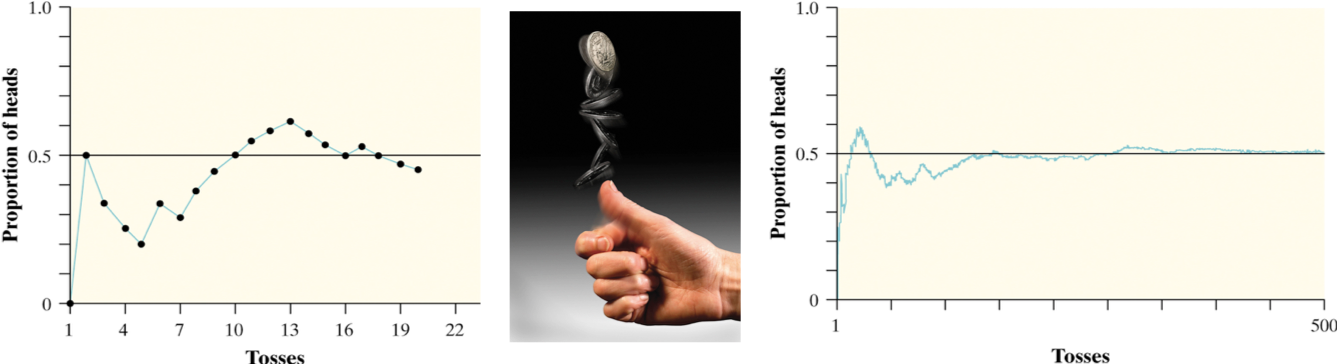
\includegraphics[width=\textwidth]{cointoss}
\end{frame}

\begin{frame}{Probability Models}
	
	\begin{itemize}
		\item We think of probability utilizing a particular framework, first we define a few useful terms
		      \begin{itemize}
		      	\item \alert{Sample Space}: set of all possible outcomes
		      	\item \alert{Event}: outcome (or set of outcomes) of a random phenomenon
		      	      \begin{itemize}
		      	      	\item Event is a subset of the sample space
		      	      \end{itemize}
		      	\item \alert{Probability Model}: assigns a probability to every event in the sample space
		      \end{itemize}
	\end{itemize}
	
\end{frame}



\begin{frame}{Probability: Example}
	
	Say we roll two six-sided die, the following would be our sample space: 
	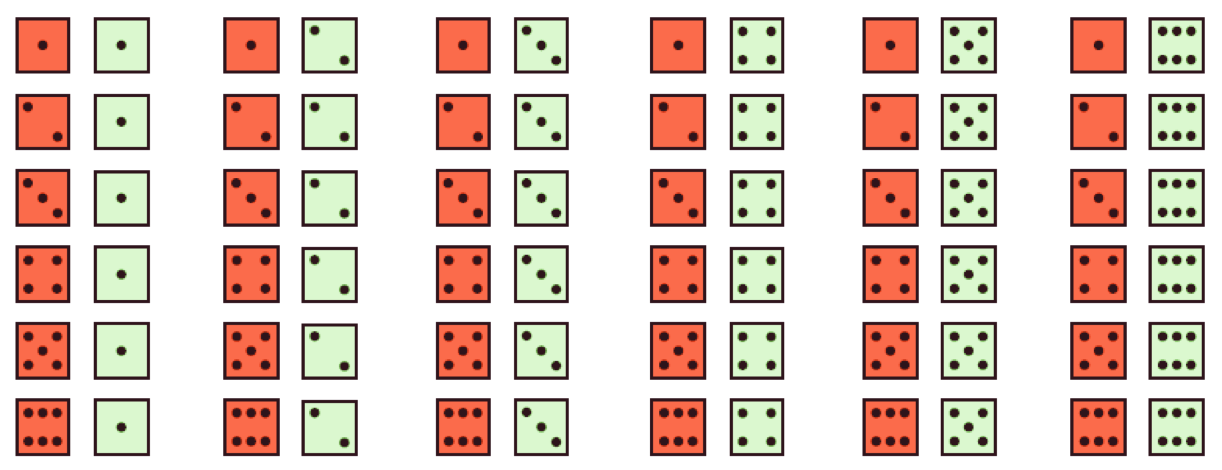
\includegraphics[width=\textwidth]{twodiesamplespace}
	\\
	Each outcome is equally likely, specifically each outcome has probability of 1/36
	
\end{frame}

\begin{frame}{Clicker Question}
	
	If I roll two six-sided die, what is the probability I roll a one and a two?
	\begin{enumerate}[label=(\alph*)]
		\item 1/36
		\item 2/36
		\item 3/36
		\item 4/36
	\end{enumerate}
	
\end{frame}

\begin{frame}{Set Notation}
	
	A =\{1,2,3\}, B=\{3,4,5\}, C=\{1,2,3,4,5,6\}, D=\{4\}
	
	\begin{itemize}
		\item $\in$: "belongs to"
		      \begin{itemize}
		      	\item Example: 1 $\in$ A
		      \end{itemize}
		\item $\notin$: "does not belong to"
		      \begin{itemize}
		      	\item Example: 4 $\notin$ A
		      \end{itemize}
		\item $\cup$: Union; combination of two or more sets; "or"
		      \begin{itemize}
		      	\item Example: A $\cup$ B = \{1,2,3,4,5\}
		      \end{itemize}
		\item $\cap$: Intersection; overlap of two or more sets; "and"
		      \begin{itemize}
		      	\item Example: A $\cap$ B = \{3\}
		      \end{itemize}
	\end{itemize}
\end{frame}


\begin{frame}{Set Notation, cont.}
	
	A =\{1,2,3\}, B=\{3,4,5\}, C=\{1,2,3,4,5,6\}, D=\{4\}
	
	\begin{itemize}
		\item $A^c$: "A complement"
		      \begin{itemize}
		      	\item Example: $A^c = {x: x \notin A} = {4}$
		      	\item Sometimes written as $A'$
		      	\item Interpreted as "not A"
		      \end{itemize}
		\item $\subseteq$: Subset
		      \begin{itemize}
		      	\item Example: $A \subseteq C$
		      	\item Everything in A is in C; not everything in C is necessarily in A
		      \end{itemize}
		\item Disjoint: $A \cap D= \emptyset$
		      \begin{itemize}
		      	\item $\emptyset$ is the null or empty set -- contains nothing 
		      \end{itemize}
	\end{itemize}
	
\end{frame}

\begin{frame}{Clicker Question}
	
	Given the following sets, A=\{5,10,15,20\} and B=\{1,2,3,4,5\}
	Which of the following is true?
	\begin{enumerate}[label=(\alph*)]
		\item $A \cup B ={1,2,3,4,5,10,15,20}$
		\item $A \cup B = {5}$
		\item $A \cap B = {5}$
		\item $A \cap B ={1,2,3,4,5,10,15,20}$
		\item Both A and C
	\end{enumerate}
	
\end{frame}

\begin{frame}{Axioms of Probability}
	
	Let A and B be events, and P(A) and P(B) are the probability of those outcomes
	\vspace{.2cm}
	\begin{itemize}
		\item Any probability is a number between 0 and 1
		\item All possible outcomes together must have the probability of 1
		      %\begin{itemize}
		      %\item If I roll a die, there is a 100\% probability I roll a 1,2,3,4,5 or 6
		      %\end{itemize}
		\item If two events are disjoint, $P(A \cap B)=0$ \\  $\hspace{45mm} \rightarrow P(A \cup B) = P(A) + P(B)$
		\item $P(A^c)=1-P(A)$
	\end{itemize}
	
\end{frame}

\begin{frame}{Clicker Question}
	Given the three following scenarios:
	\begin{itemize}
		\item A person is randomly selected. A is the event they are under 18. B is the event they are over 18.
		\item A person is selected at random. A is the event that they earn more than \$100,000 per year. B is the event that they earn more than \$250,000.
		\item A pair of dice are tossed. A is the event that one of the die is a 3. B is the event that the sum of two dice is 3.
	\end{itemize}
	\vspace{.2cm}
	In which cases are the events, A and B, disjoint?
	\begin{center}
		\begin{columns}
			\column{0.5\textwidth}
			\begin{itemize}
				\item[(a)] 1 only
				\item[(b)] 2 only
				\item[(c)] 3 only
			\end{itemize}
			\column{0.5\textwidth}
			\begin{itemize}
				\item[(d)] 1 and 2
				\item[(e)] 1 and 3
			\end{itemize}
		\end{columns}
	\end{center}
\end{frame}



\begin{frame}{De Morgan's Law}
	De Morgan's law of  union and intersection
	\begin{itemize} 
		\item For any two finite sets A and B:
		      \begin{itemize}
		      	\item[(i)] $(A \cup B)^c = A^c \cap B^c$
		      	\item[(ii)] $(A \cap B)^c = A^c \cup B^c$
		      \end{itemize}
	\end{itemize}
	
\end{frame}

\begin{frame}{De Morgan's Law Example}
	Let S=\{j, k, l, m, n\} and A=\{j, k, m\} and B=\{k, m, n\}
	\begin{itemize}
		
		\item[(i)]
		      $(A \cup B)= \{j, k, m, n\} \implies (A \cup B)^c=\{l\}$ \hspace{14mm} (1)
		      
		      $A^c = \{l, n\} \text{ and }B^c=\{j, l\} \implies A^c \cap B^c = \{l\}$ \hspace{8mm} (2)
		      \begin{itemize}
		      	
		      	\item (1) and (2) imply $(A \cup B)^c = (A^c \cap B^c)$
		      \end{itemize}
		      
		\item[(ii)] 
		      $(A \cap B)=\{k,m\} \implies (A \cap B)^c=\{j, l, n\}$ \hspace{14mm} (1) 
		      
		      $A^c \cup B^c=\{l, n\} \cup \{j, l\} \implies A^c \cup B^c = \{j, l, n\}$ \hspace{4mm} (2) 
		       
		      \begin{itemize}
		      	\item (1) and (2) imply $(A \cap B)^c = A^c \cup B^c$
		      \end{itemize}
	\end{itemize}
\end{frame}



\begin{frame}{Random Variables}
	
	\begin{itemize}
		\item \alert{Random variable}: variable whose value is a numerical outcome of a random phenomenon
		      \begin{itemize}
		      	\item Random variables can be discrete or continuous
		      \end{itemize}
		\item Coin toss example
		      \begin{itemize}
		      	\item X can be defined as the number of heads we see in two tosses:
		      	      \begin{itemize}
		      	      	\item X is a discrete random variable; X=0,1,2
		      	      \end{itemize}
		      \end{itemize}
		\item \alert{Probability distribution}: tell us what values random variable X can take, and how to assign probabilities to those values
	\end{itemize}
	
\end{frame}

\begin{frame}{Example}
	
	Flip a coin two times
	\begin{itemize}
		\item State space:
		      \begin{itemize}
		      	\item (Head, Tail), (Head, Head), (Tail, Head), (Tail, Tail)
		      \end{itemize}
		\item What is the probability of each event?
	\end{itemize}
	
\end{frame}

\begin{frame}{Clicker Question}
	
	If I toss a coin two times, and X is the number of heads, then what is P(X=2)?
	\begin{enumerate}[label=(\alph*)]
		\item 1/4
		\item 1/2
		\item 3/4
		\item 5/4
	\end{enumerate}
	
\end{frame}

\begin{frame}{Additional Examples}
	
	\begin{itemize}
		\item  Still flipping a coin twice, what is the probability of getting at least one head?
		      \begin{itemize}
		      	\item $P(X=1) + P(X=2) = 1-P(X=0)$
		      \end{itemize}
	\end{itemize}
	
\end{frame}

\begin{frame}{Additional Dice Example}
	What is the probability of rolling a 7, 11, or double when rolling two dice?
	
	Axiom 3 tells us we can find probabilities simply by adding if the event is disjoint (we'll talk more Friday about what to do when events are not disjoint).
	
	Are all 3 events disjoint?
\end{frame}

\begin{frame}{Additional Dice Example}
	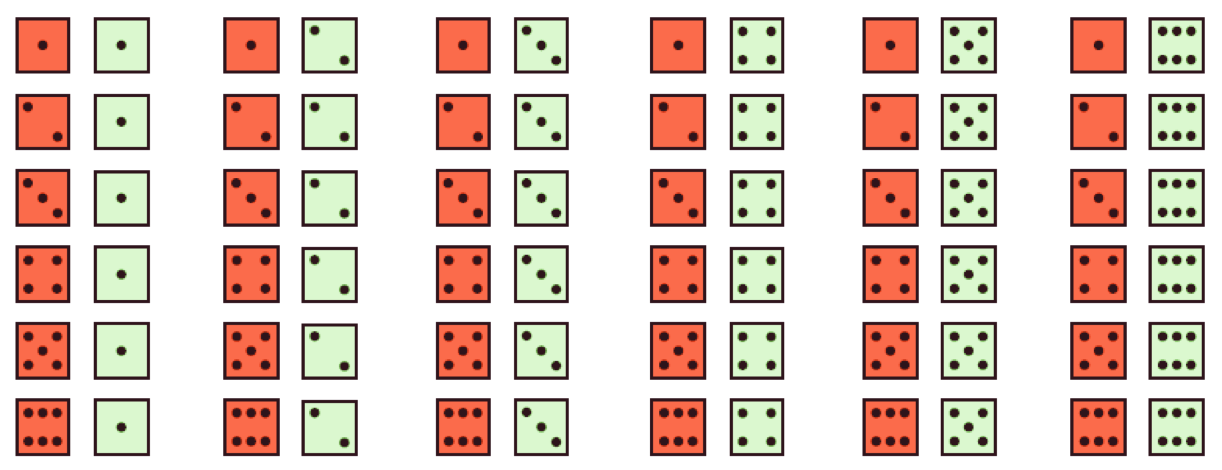
\includegraphics[width=\textwidth]{twodiesamplespace}
	
	$P(7)+P(11)+P(doubles)=\frac{6}{36}+\frac{2}{36}+\frac{6}{36} \approx 0.4$
\end{frame}




\end{document}